\chapter{Technical Background}

Over the course of the past decade, elliptic curve cryptography (ECC) has proven itself a mainstay in the wide world of applied cryptology. While isogeny based cryptography does build itself up from the same underlying field of mathematics as ECC, it simultaneously draws from a slightly more complicated space of algebraic notions. Much of this chapter will be dedicated to illuminating these notions in a manner that should be digestable for those without serious background in algebraic geometry, or abstract algebra in general.

This chapter will cover the following preliminary topics: isogenies and their relevant properties, supersingular isogeny Diffie-Hellman (SIDH) and related procotols, the Fiat-Shamir construction for digital signatures (and its quantum-safe adaptation), and finally the current landscape of isogeny based signature schemes.

Our discussion of isogenies will begin with some basic coverage of the underlying algebra. We will provide the material necessary for the remaining sections as we build up in the level of abstraction; working our way through groups, finite fields, elliptic curves, and finally isogenies and their properties.

Once we have presented the necessary algebra, we will illustrate the specifics of the supersingular isogeny Diffie-Hellman key-exchange protocol. We will spend most of this time dedicated to a modular deconstruction of the protocol, reviewing the underlying isogeny-level procedures and algorithms which will be necessary for understanding in detail the signature protocol to come. Another task of this section will be to introduce the SIDH C library released by Microsoft Research, on top of which the core contributions of this thesis are implemented. This subsection will end with a briefing and analysis of the closely related zero-knowledge proof of identity (ZKPoI) isogeny protocol proposed in the original De Feo et al. paper[ref], as it is necessary for understanding the isogeny based signature scheme presented by Yoo et al[ref].

In section 2.3 we will discuss the Fiat-Shamir transformation; a technique which, given a secure interactive proof of knowledge, creates a secure digital signature scheme. We will also look at the quantum-secure adaptation published by Unruh, for applying a non-quantum-resistant transform to a quantum-resistant primitive would be rather frivolous.

Finally, the last section of this chapter will be dedicated to covering current isogeny-based signature schemes - the topic of which this dissertation is mainly concerned. We will primarily discuss the signature scheme of Yoo et al., which is a near direct application of Unruh's Fiat-Shamir adaptation to the SIDH zero-knowledge proof of identity to be discussed at the end of section 2.2.\\

\section{Algebraic Geometry \& Isogenies}
\emph{Groups \& Varieties}. A \textbf{group} is a 2-tuple composed of a set of elements and a corresponding group operation (also referred to as the group \emph{law}). Given some group defined by the set $G$ and the operation $\cdot$ (written as $(G,\cdot)$) it is typical to refer to the group simply as $G$. If $\cdot$ is equivalent to some rational mapping[footnote about rational mappings] $f_G: G \rightarrow G$, then the group $(G,\cdot)$ is said to form an \textit{algebraic variety}[footnote about the inverse function]. A group which is also an algebraic variety is referred to as an \textbf{algebraic group}.

$G$ is said to be an \emph{abelian} group if, in addition to the four traditional group axioms (closure, associativity, existence of an identity, existence of an inverse), $G$ satisfies the condition of commutitiviy. More formally, for some group $G$ with group operation $\cdot$, we say $G$ is an abelian group iff $x \cdot y = y \cdot x$ $\forall x, y \in G$. An algebraic group which is also abelian is referred to as an \textbf{abelian variety}.

\begin{tcolorbox}
\begin{definition}[Abelian Variety]
\label{defn:abelianvariety}
for some algebraic group $G$ with operation $\cdot$, we say $G$ is an \underline{abelian variety} iff $x \cdot y = y \cdot x$ $\forall x, y \in G$. 
\end{definition}
\end{tcolorbox}

For some group $(G,\cdot)$, some $x,y \in G$, and some rational mapping $f_G: G \rightarrow G$, let the following sequence of implications denote the classification of $(G,\cdot)$:

$$
\text{group } \xRightarrow[]{x\cdot y = f_G(x,y)} \text{algebraic group } \xRightarrow[]{x\cdot y = y\cdot x} \text{abelian variety }
$$


\noindent
\emph{Morphisms}. Let us again take for example some group $(G,\cdot)$. Let's also define some set $S_{(G,\cdot)}$ which contains every tuple $(x,y,z)$ for group elements $x,y,z$ which satisfy $x\cdot y = z$.
$$
S_{(G,\cdot)} = \{x,y,z \in G | x\cdot y = z\}
$$
Take also for example a second group $(H,*)$ and some map $\phi: G \rightarrow H$. $\phi$ is said to be \emph{structure preserving} if the following implication holds:
$$
(x,y,z) \in S_{(G,\cdot)} \Rightarrow (\phi(x),\phi(y),\phi(z)) \in S_{(H,*)}
$$

A \textbf{morphism} is simply the most general notion of a structure preserving map. More specifically, in the domain of algebraic geometry, we will be dealing with the notion of a \textbf{group homomorphism}, defined as follows:
\begin{tcolorbox}
\begin{definition}[Group Homomorphism]
\label{defn:homomorphism}
For two groups $G$ and $H$ with respective group operations $\cdot$ and $*$, a \underline{group homomorphism} is a structure preserving map $h: G \rightarrow H$ such that $\forall u, v \in G$ the following holds:
$$h(u \cdot v) = h(u) * h(v)$$
\end{definition}
\end{tcolorbox}

From this simple definition, two more properties of homomorphisms are easily deducible. Namely, for some homomorphism $h: G \rightarrow H$, the following properties hold:
\begin{itemize}
\item $h$ maps the identity element of $G$ onto the identity element of $H$, and
\item $h(u^{-1}) = h(u)^{-1}, \forall u \in G$
\end{itemize}

Furthermore, an \textbf{endomorphism} is a special type of morphism in which the domain and the codomain are the same groups.
\begin{tcolorbox}
\begin{definition}[Endomorphism]
\label{defn:endomorphism}
For two groups $G$ and $H$, an \underline{endomorphism} is a morphism $\psi: G \rightarrow H$ wherein $G = H$
\end{definition}
\end{tcolorbox}

\noindent
\emph{Fields \& Field Extensions}. An algebraic group $G_a$ is defined over a field $K$ if each element $e \in G_a$ is defined over $K$ and the corresponding $f_{G_a}$ is also defined over $K$. To show that a particular algebraic group $G_a$ is defined over some field $K$ we will henceforth denote the group/field pairing as $G_a(K)$.\\

\noindent
\emph{Quotient Groups}.

These algebraic structures are all important for building up to the concept of an \emph{isogeny}. The lowest-level structure we will be concerned with when discussing the forthcoming isogeny-based protocols will typically be abelian varieties. The lowest-level structure in the SIDH C codebase is a finite field element.\\

\subsection{Elliptic Curves}

An elliptic curve is an algebraic curve defined over some field $K$, the most general representation of which is given by
$$
y^2 + a_{1}xy + a_{3}y = x^3 + a_{2}x^2 + a_{4}x + a_6.
$$
This representation encapsulates elliptic curves defined over any field. If, however, we are dicussing curves defined specifically over a field $K$ such that $\text{char}(K) > 3$[ref], then the more compact form $y^2 = x^3 + ax + b$ can be applied. In this dissertation we will default to this second representation, as the schemes with which we are concerned will always be defined over $\mathbb{F}_p$ for some large prime $p$.

Within algebraic geometry, it is common practice to define a group structure over the points of a given elliptic curve (or any other smooth cubic curve). If we wish to define a group in accordance to a particular curve, we do so with the following notation:
$$
E: y^2 = x^3 + ax + b
$$
Wherein $E$ denotes the group in question, the elements of which are all the points (solutions) of the curve. Throughout much of this section, the words \emph{point} and \emph{element} can be used interchangeably.\\

\noindent
\emph{The Group Law}. The group operation we define for $E$, denoted $+$, is better understood geometrically than algebraically. Consider the following.

Given two elements $P$ and $Q$ of some arbitrary elliptic curve group $E$, we define $+$ geometrically as follows: drawing the line $L$ formed by points $P$ and $Q$, we follow $L$ to its third intersection on the curve, which we will denote as $R = (x_R, y_R)$. We then set $P + Q = -R$, where $-R$ is the reflection of $R$ over the x-axis: $(x_R, -y_R)$. See figure [fig] for an illustrated representation of this process.

\begin{figure}[!h]
\begin{tikzpicture}[scale=.75]
	\begin{scope}[xshift=5cm]
		%\draw[very thin,color=gray] (-3.9,-3.9) grid (3.9,3.9);  %background grid
		\draw[->] (-4.2,0) -- (4.2,0) node[right] {$x$};         %x-axis
		\draw[->] (0,-4.2) -- (0,4.2) node[above] {$y$};         %y-axis
		
		\plotcurve{-2}{2}
		
		\draw[fill] (-1.73,0.531) circle (0.1) node[right] {$P$};
		\draw[fill] (0.28,1.209) circle (0.1) node[right] {$Q$};
	\end{scope}
	
	\begin{scope}[xshift=17cm]
		%\draw[very thin,color=gray] (-3.9,-3.9) grid (3.9,3.9);  %background grid
		\draw[->] (-4.2,0) -- (4.2,0) node[right] {$x$};         %x-axis
		\draw[->] (0,-4.2) -- (0,4.2) node[above] {$y$};         %y-axis
		
		\plotcurve{-2}{2}
		
		\draw [] (-1.73,0.531) -- (1.564,1.642);
		\draw [dashed] (1.564,1.642) -- (1.564,-1.642);
		
		\draw[fill] (-1.73,0.531) circle (0.1) node[right] {$P$};
		\draw[fill] (0.28,1.209) circle (0.1) node[right] {$Q$};
		\draw[fill] (1.564,1.642) circle (0.1) node[right] {$R$};
		\draw[fill] (1.564,-1.642) circle (0.1) node[right] {$R' = P+Q$};
  \end{scope}
\end{tikzpicture}
\caption{$+$ acting over points $P$ and $Q$ of $y^2 = x^3 - 2x + 2$.}
\label{fig:groupop}
\end{figure}

The group operation $+$ is referred to as \emph{pointwise addition}. In order for $(E,+)$ to properly form a group under pointwise addition, it must satisfy the four group axioms:
\begin{itemize}
\item \emph{Closure}: Because elliptics curves are polynomials of degree of 3, we know any given line passing through two points $P$ and $Q$ of $E$ will pass through a third point $R$. The exceptions here are twofold. First, when $P = Q$ and thus our line is tangent to $E$, and second, when $Q = -P$ and our line is parallel with the y-axis. We resolve the first case nicely by defining $P + P$ by means of taking $L$ to be the line tangent to $E$ at point $P$. In the second case, $P + (-P)$, by group axiom, should yield the identity element of the group. We will define this element and resolve this issue below.  
\item \emph{Identity}: The identity element of elliptic curve groups, denoted as $\mathcal{O}$, is a specially defined point satisfying $P + \mathcal{O} = \mathcal{O} + P = P$, $\forall P \in E$. Because of the inclusion of this special element, we have that $\#(E(K))$ is equal to $1$ $+$ the number geometric points on $E$ defined over $K$. This of course is only a noteworthy claim when $K$ is a finite field (otherwise there are already infinitely many elements in $E$).
\item \emph{Associativity}: To show that associativity holds for geometrically defined points $P$, $Q$, and $R$ in $E$ ($(P + Q) + R = P + (Q + R)$) is rather simple (see figure [fig]). We can also show that this holds when any combination of $P$, $Q$, and $R$ are $\mathcal{O}$ by simply applying the axiom of the identity.
\item \emph{Inverse}: Because elliptic curves are symmetrical about the x-axis, every point $P$ of $E$ inverse element of $P$ to be $-P$, defined the same as above. It is easy to see that $P+(-P) = \mathcal{O}$ Because of this, $\mathcal{O}$ can be thought of as a point residing infinitely far in both the positive and negative directions of the y-axis. $\mathcal{O}$ is equivalently referred to as the \emph{point at infinity}.
\end{itemize}

\begin{figure}[!h]
\begin{tikzpicture}[scale=.60]
	\begin{scope}[xshift=0cm]
		%\draw[very thin,color=gray] (-3.9,-3.9) grid (3.9,3.9);  %background grid
		\draw[->] (-4.2,0) -- (4.2,0) node[right] {$x$};         %x-axis
		\draw[->] (0,-4.2) -- (0,4.2) node[above] {$y$};         %y-axis
		
		\plotcurve{-3}{0}
		
		\draw[fill] (-1.73,0.531) circle (0.1) node[right] {$P$};
		\draw[fill] (0.28,1.209) circle (0.1) node[right] {$Q$};
	\end{scope}
	
	\begin{scope}[xshift=10cm]
		%\draw[very thin,color=gray] (-3.9,-3.9) grid (3.9,3.9);  %background grid
		\draw[->] (-4.2,0) -- (4.2,0) node[right] {$x$};         %x-axis
		\draw[->] (0,-4.2) -- (0,4.2) node[above] {$y$};         %y-axis
		
		\plotcurve{-3}{0}
		
		\draw[fill] (-1.73,0.531) circle (0.1) node[right] {$P$};
		\draw[fill] (0.28,1.209) circle (0.1) node[right] {$Q$};
	\end{scope}
	
	\begin{scope}[xshift=20cm]
		%\draw[very thin,color=gray] (-3.9,-3.9) grid (3.9,3.9);  %background grid
		\draw[->] (-4.2,0) -- (4.2,0) node[right] {$x$};         %x-axis
		\draw[->] (0,-4.2) -- (0,4.2) node[above] {$y$};         %y-axis
		
		\plotcurve{1}{1}
		
		\draw [dashed] (0.73,-4.492) -- (0.73,4.492);
		
		\draw[fill] (0.73,1.492) circle (0.1) node[right] {$P$};
		\draw[fill] (0.73,-1.492) circle (0.1) node[right] {$-P$};
  \end{scope}
\end{tikzpicture}
\caption{associativity illustrated on $y^2 = x^3 - 3x$ (left \& center) and $P + (-P) = \mathcal{O}$ illustrated for $y^2 = x^3 + x + 1$ (right).}
\label{fig:groupop}
\end{figure}

Additionally, we shorthand $\overbrace{P + P + ... + P}^{n}$ as $nP$, analogous to scalar multiplication.\\

Consequently, because groups defined over elliptic curves in this fashion are commutitive, they also constitute abelian varieties[ref].

When referring to curves as abelian varieties defined over a field, we will write them as $E_{\alpha}(K)$, for some curve $E_{\alpha}$ and some field $K$. If we are only concerned with the geometric properties of the curve, or curves as distinct elements of some group structure, it will suffice to write $E_{\alpha}$. Moving forward from here, we will assume all general curves discussed are capable of definition over some finite field $\mathbb{F}_p$.\\

\noindent
\emph{Torsion Groups}. The $r$-\emph{torsion group} of $E$ is the set of all points $P \in E(\overline{\mathbb{F}}_q)$ such that $[r]P = \mathcal{O}$. We denote the $r$-torsion group of some curve as $E[r]$.\\

\noindent
\emph{Supersingular Curves}. An elliptic curve can be either \emph{ordinary} or \emph{supersingular}. There are several equivalent ways to define supersingular curves (and thus the distinction between them and ordinary curves,)

For the remainder of this paper, unless otherwise noted, all elliptic curves in discussion will be of the supersingular variety.

\subsection{Isogenies \& Their Properties}

\begin{tcolorbox}
\begin{definition}[Isogeny]
\label{defn:isogeny}
Let $G$ and $H$ be algebraic groups[ref]. An \underline{isogeny} is a morphism[ref] $h: G \rightarrow H$ possessing a finite kernel.
\end{definition}
\end{tcolorbox}

In the case of the above definition where $G$ and $H$ are abelian varieties (such as elliptic curves,) the isogeny $h$ is homomorphic[ref] between $G$ and $H$. Because of this, isogenies over elliptic curves (and other abelian varieties) inherit certain characteristics.\\
For an isogeny $h: E_{1} \rightarrow E_{2}$ defined over elliptic curves $E_1$ and $E_2$, the following holds:
\begin{itemize}
\item $h(\mathcal{O}) = \mathcal{O}$, and
\item $h(u^{-1}) = h(u)^{-1}, \forall u \in G$
\end{itemize}

We write $\text{End}(E)$ to denote the ring formed by all the isogenies acting over $E$ which are also endomorphisms. Note that $m$-repeated pointwise addition of a point with itself can equivalently be modelled by an endomorphism, we denote the application of such an endomorphism to a point $P$ as $[m]P$, such that $[m]: E \rightarrow E$ and $[m]P = mP$.

\section{Supersingular Isogeny Diffie-Hellman}

This section will aim to accomplish two things. First, we will briefly explain the isogeny-level \& key-exchange-level procedures of the SIDH protocol. Second, we will illuminate how these procedures map onto Microsoft Research's C implementation of SIDH. In this regard, this section can be considered an attempt to meld two domains of SIDH functions \& procedures, in hopes of easing the navigation from the SIDH protocol to Microsoft's C implementation, and vice versa.

The original work of De Feo, Jao, and Plut outlines three different isogeny-based cryptographic primitives: Diffie-Hellman-esque key exchange, public key encryption, and the aforementioned zero-knowledge proof of identity. Because all three of these protocols require the same initialization and public parameters, we will begin by covering these parameters in detail. Immediately after, we will analyze the key exchange at a relatively high level. Our goal of this section is to explain in detail the algorithmic and cryptographic aspects of the ZKPoI scheme, as this forms the conceptual basis for the signature scheme we will be investigating. We begin with the key exchange protocol because its sub-routines are integral to the Yoo et. Al signature implementation.

For the discussion that follows, we will assume every instance of an SIDH protocol occurs between two parties, \textcolor{blue}{A} and \textcolor{red}{B} (eg. \textcolor{blue}{Alice} \& \textcolor{red}{Bob},) for which we will colorize information particular to \textcolor{blue}{A} in \textcolor{blue}{blue} and \textcolor{red}{B} in \textcolor{red}{red}. This will include private keys \& public keys as well as the variables and constants used in their generation.

\subsection{Public Parameters}

As the name suggests, SIDH protocols work over supersingular curves (of a smooth order). Let $\mathbb{F}_q = \mathbb{F}_{p^2}$ be the finite field over which our curves are defined, $\mathbb{F}_{p^2}$ denoting the quadratic extension field of $\mathbb{F}_{p}$.  $p$ is a prime defined as follows:
$$
p = \laea \lbeb \cdot f \pm 1
$$
Wherein $\la$ and $\lb$ are small primes (typically \textcolor{blue}{2} \& \textcolor{red}{3}, respectively) and $f$ is a cofactor ensuring the primality of $p$. We then define a global parameter curve $E$ defined over $\mathbb{F}_q$ with cardinality $(\laea \lbeb f)^2$. Consequently, the torsion group $E[\laea]$ is $\mathbb{F}_q$-rational and has $\la^{\ea - 1} (\la + 1)$ cyclic subgroups of order $\laea$, with the analogous statement being true for $E[\lbeb]$.

Additionally, we include in the public parameters the bases $\{P_A,Q_A\}$ and $\{P_B,Q_B\}$, generating $E[\laea]$ and $E[\lbeb]$ respectively.\\

\subsection{SIDH Key Exchange}

This subsection will illustrate an SIDH key exchange run between party members \textcolor{blue}{Alice} and \textcolor{red}{Bob}. The general idea of the protocol can be surmised by the diagram below. In the scheme, \textbf{private keys} take the form of isogenies[ref] defined with domain $E$, and \textbf{public keys} are the associated co-domain curve of said isogenies.

\begin{center}
\begin{tikzpicture}
  \matrix (m) [matrix of math nodes,
               row sep=4em,
               column sep=4em,
               minimum width=2em] {
    E                     & E / \langle \textcolor{blue}{A} \rangle    \\
    E / \langle \textcolor{red}{B} \rangle & E / \langle \textcolor{blue}{A}, \textcolor{red}{B} \rangle \\
  };
  \path[-stealth]
    (m-1-1) edge node [above] {$\pa$}  (m-1-2)
    (m-1-1) edge node [left]  {$\pb$}  (m-2-1)
    (m-2-1) edge node [below] {$\pap$} (m-2-2)
    (m-1-2) edge node [right] {$\pbp$} (m-2-2);
\end{tikzpicture}
\end{center}

\noindent
\textit{Key Generation}. \textcolor{blue}{Alice} chooses two random numbers $m_A, n_A \in \mathbb{Z}/\laea\mathbb{Z}$ such that $(\la \nmid m_A) \lor (\la \nmid n_A)$. Following this, \textcolor{blue}{Alice} computes the isogeny $\phi_A: E \rightarrow E_A$ with kernel $K_A := \langle [m_A]P_A, [n_A]Q_A\rangle$.\\


\noindent
\textit{PK Exchange}. In addition to sending their respective isogenies,\\

\noindent
\textit{Secret Agreement}.\\

\begin{figure}[htb]
\centering
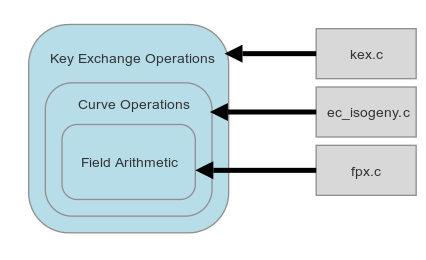
\includegraphics[scale=0.7]{halfmapwcurve.png} % e.g. insert ./image for image.png in the working directory, adjust scale as necessary
\caption{Relationship between SIDH key exchange \& MR SIDH C library}
\label{fig:halfmap} % insert suitable label, this is used to refer to a fig from within the text as shown above
\end{figure}

\subsection{Modular Breakdown}

Figure [ref] illustrates the relationship between abstraction levels of the SIDH protocol and modules of the SIDH C library.

\begin{figure}[htb]
\centering
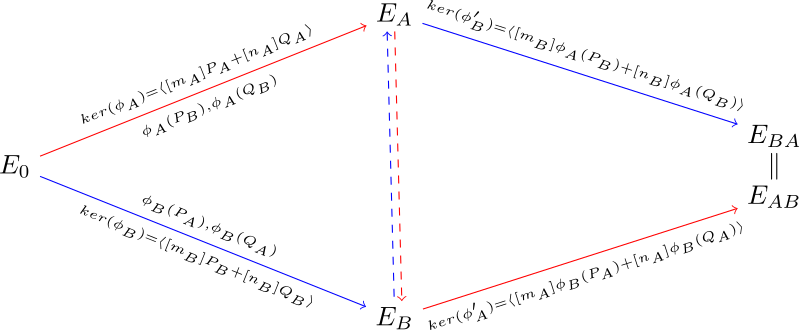
\includegraphics[scale=0.5]{keyexchange.png} % e.g. insert ./image for image.png in the working directory, adjust scale as necessary
\caption{SIDH key exchange between \textcolor{blue}{Alice} \& \textcolor{red}{Bob}}
\label{fig:kex} % insert suitable label, this is used to refer to a fig from within the text as shown above
\end{figure}


\subsection{Security Assumptions}



\subsection{Zero-Knowledge Proof of Identity}

Recall the notion of a simple identification scheme:

\section{Fiat-Shamir Construction}

The Fiat-Shamir construction (sometimes referred to as the Fiat-Shamir heuristic or transform) is used

\subsection{Unruh's Post-Quantum Adaptation}



\section{Isogeny Based Signatures}

Now that we've introduced the zero-knowledge proof of identity scheme from [REFERENCE] as well as Unruh's quantum-safe Fiat-Shamir adaption, the isogeny based signature scheme presented by Yoo et. Al is a near-trivial application of the latter to the former. 

The isogeny based signature scheme presented by Yoo et. Al is defined, in the traditional manner, by a tuple of algorithms. Namely, the scheme is defined by the tuple (KeyGen, Sign, Verify) with each algorithm loosely defined as follows:\\
\textbf{KeyGen(}\textbf{)}: Select a random point $S$ of order $\ell_{A}^{e_A}$, compute the isogeny $\phi: E \rightarrow E/ \langle S \rangle$. Return (pk, sk) where pk = $(E/ \langle S \rangle, \phi(P_B), \phi(Q_B))$ and sk = $S$.\\
\textbf{Sign()}:\\
\textbf{Verify()}:\\

\subsection{Modular Breakdown}

\begin{figure}[htb]
\centering
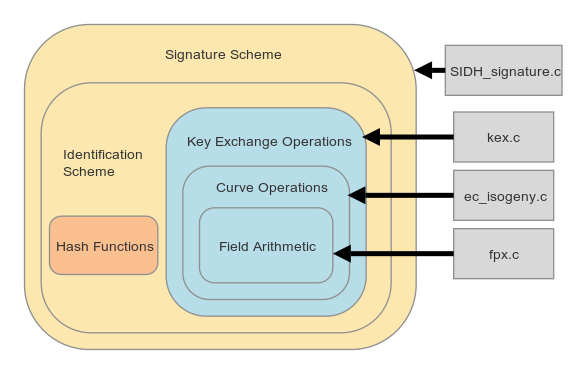
\includegraphics[scale=0.7]{fullmapwcurve.png} % e.g. insert ./image for image.png in the working directory, adjust scale as necessary
\caption{Relationship between SIDH based signatures \& Our fork of the SIDH C library}
\label{fig:fullmap} % insert suitable label, this is used to refer to a fig from within the text as shown above
\end{figure}


Shortly after, the following, more in-depth algorithms are given as definitions: 

\begin{algorithm}
\caption{KeyGen($\lambda$)}\label{euclid}
\begin{algorithmic}[1]
\State Pick a random point S of order $\ell^{e_{A}}_{A}$
\State Compute the isogeny $\phi: E \rightarrow E/\langle S \rangle$
\State pk $\gets (E/\langle S \rangle, \phi(P_{B}), \phi(Q_{B}))$
\State sk $\gets S$
\State \Return (pk,sk)
\end{algorithmic}
\end{algorithm}

\begin{algorithm}
\caption{Sign(sk, $m$)}\label{euclid}
\begin{algorithmic}[1]
\For{\texttt{i = 1..2$\lambda$}}
	\State Pick a random point R of order $\ell^{e_{B}}_{B}$
	\State Compute the isogeny $\psi: E \rightarrow E/\langle R \rangle$
	\State Compute either $\phi' : E/\langle R \rangle \rightarrow E/\langle R,S \rangle$ or $\psi' : E/\langle S \rangle \rightarrow E/\langle R,S \rangle$
	\State $(E_{1},E_{2}) \gets (E/\langle R \rangle, E/\langle R,S \rangle)$
	\State $\texttt{com}_{i} \gets (E_{1}, E_{2})$
	\State $\texttt{ch}_{i,0} \gets_{R} \{0,1\}$
	\State $(\texttt{resp}_{i,0}, \texttt{resp}_{i,1}) \gets ((R,\phi(R)), \psi(S))$
	\If{$\texttt{ch}_{i,0} = 1$}
		\State $\texttt{swap}(\texttt{resp}_{i,0},\texttt{resp}_{i,1})$
	\EndIf
	\State $h_{i,j} \gets G(\texttt{resp}_{i,j})$
\EndFor

\State $J_{1} \parallel ... \parallel J_{2\lambda} \gets H(pk, m, (\texttt{com}_{i})_{i},(\texttt{ch}_{i,j})_{i,j},(h_{i,j})_{i,j})$

\State \Return $\sigma \gets ((\texttt{com}_{i})_{i}, (\texttt{ch}_{i,j})_{i,j}, (h_{i,j})_{i,j}, (\texttt{resp}_{i,J_{i}})_{i})$
\end{algorithmic}
\end{algorithm}

\begin{algorithm}[H]
\caption{Verify(pk, $m$, $\sigma$)}\label{euclid}
\begin{algorithmic}[1]
\State $J_{1} \parallel ... \parallel J_{2\lambda} \gets H(pk, m, (\texttt{com}_{i})_{i},(\texttt{ch}_{i,j})_{i,j},(h_{i,j})_{i,j})$
\For{\texttt{i = 0..2$\lambda$}}
	\State \textbf{check} $h_{i,J_{i}} = G(\texttt{resp}_{i,J_{i}})$
	\If{$\texttt{ch}_{i,J_{i}} = 0$}
		\State Parse $(R,\phi(R)) \gets \texttt{resp}_{i,J_{i}}$
		\State \textbf{check} $(R, \phi(R))$ have order $\ell^{e_{B}}_{B}$
		\State \textbf{check} $R$ generates the kernel of the isogeny $E \rightarrow E_{1}$
		\State \textbf{check} $\phi(R)$ generates the kernel of the isogeny $E/\langle S \rangle \rightarrow E_{2}$
	\Else
		\State Parse $\psi(S) \gets \texttt{resp}_{i,J_{i}}$
		\State \textbf{check} $\psi(S)$ has order $\ell^{e_{A}}_{A}$
		\State \textbf{check} $\psi(S)$ generates the kernel of the isogeny $E_{1} \rightarrow E_{2}$
	\EndIf
\EndFor

\If{all checks succeed}
	\State \Return 1
\EndIf
\end{algorithmic}
\end{algorithm}

If we transcribe the above to the language of the Microsoft SIDH API, we have in essense the following:\\

\begin{algorithm}
\caption{KeyGen($\lambda$)}\label{euclid}
\begin{algorithmic}[1]
\State (pk, sk) $\gets \texttt{KeyGeneration\_B()}$
\State \Return (pk,sk)
\end{algorithmic}
\end{algorithm}

\begin{algorithm}
\caption{Sign(sk, $m$)}\label{euclid}
\begin{algorithmic}[1]
\For{\texttt{i = 1..2$\lambda$}}
	\State $(, R, \psi) \gets \texttt{KeyGeneration\_A(E)}$
	\State $E_{1} \gets E/\langle R \rangle$
	\State $(E_{2},E/\langle R,S \rangle) \gets \texttt{SecretAgreement\_B()}$
	\State $(E_{1},E_{2}) \gets (E/\langle R \rangle, E/\langle R,S \rangle)$
	\State $\texttt{com}[i] \gets (E_{1}, E_{2})$
	\State $\texttt{ch}[i] \gets_{R} \{0,1\}$
	\State $(\texttt{resp}[i]_{0}, \texttt{resp}[i]_{1}) \gets ((R,\phi(R)), \psi(S))$
	
%% this portion was skipped?	
%%	\If{$\texttt{ch}[i] = 1$}
%%		\State $\texttt{swap}(\texttt{resp}[i]_{0},\texttt{resp}[i]_{1})$
%%	\EndIf
%%	\State $h_{i,j} \gets G(\texttt{resp}[i]_{j})$
\EndFor

\State $J_{1} \parallel ... \parallel J_{2\lambda} \gets H(pk, m, (\texttt{com}_{i})_{i},(\texttt{ch}_{i})_{i},(h_{i,j})_{i,j})$

\State \Return $\sigma \gets ((\texttt{com}_{i})_{i}, (\texttt{ch}_{i,j})_{i,j}, (h_{i,j})_{i,j}, ((\texttt{resp})[J_{i}])$
\end{algorithmic}
\end{algorithm}
